


\documentclass[14pt]{report}

\usepackage{url,amssymb, amsmath,color}

\usepackage{fontspec}                     %加這個就可以設定字體
\setmainfont{Noto Sans CJK JP}                  %直接設定Windows中的字型,名字要打的一模一樣才行。
\XeTeXlinebreaklocale "zh"                %這兩行一定要加,中文才能自動換行
\XeTeXlinebreakskip = 0pt plus 1pt   

\usepackage{graphicx}


\title{\Huge Pattern Recognition}
\author{\huge Homework 1  \\ \\王淮慕\\學號 : 606415050\\系所 : 電機系}
\date{\today}
\begin{document}
	
	\maketitle
	
	\section{Consider the minimax criterion for a two-category classification problem.}
	\begin{enumerate}
		\item Assume $p(x|\omega_1) = \sim N(0,1)$ and $p(x|\omega_2) = \sim N(1/2,1/4)$ under a zero-one loss. Find the decision threshold $x^\ast$ and the resulting overall risk .
		\item [1-1] sol :\\
		\[\int_{R_2}^{}p(x|\omega_1)dx=\int_{R_1}^{}p(x|\omega_2)dx \]
		\[\Rightarrow \int_{\theta}^{\infty}\frac{1}{\sqrt{2\pi}}\exp [\frac{-1}{2}x^2]dx
		=\int_{-\infty}^{\theta}\frac{1}{\sqrt{2\pi}\times \frac{1}{2}}\exp [\frac{-1}{2\times \frac{1}{2}}(x-\frac{1}{2})^2]dx \]
		\[\Rightarrow \Phi(-\theta)=\Phi(\frac{\theta-\frac{1}{2}}{\frac{1}{2}}) \]
		\[\Rrightarrow \-\theta=\frac{\theta-\frac{1}{2}}{\frac{1}{2}} \]
		\[\color{red} \Rrightarrow \theta =1\]
		\item [1-2] sol :\\
		\[R=\int_{R_1}^{}p(x|\omega_2)dx\]
		\[=\int_{-\infty}^{1}p(x|\omega_2)dx\]
		\[=\Phi(\frac{1-\frac{1}{2}}{\frac{1}{2}})\]
		\[=\Phi(-1)\]
		\[\color{red} =0.1587\]
	\end{enumerate}
	
	\section{Consider the Neyman-Person criterion for two univariate normal distributions : \\ $p(x|\omega_1) \sim N(-1,2) , p(x|\omega_2) \sim N(2,4)\\and\ P(\omega_1)=0.6$.}
	\begin{enumerate}
		\newpage
		\item Suppose the maximum acceptable error rate for classifying a pattern that is actually in $\omega_1$ as if it were in $\omega_2$ is 0.05. What is the resulting single-point decision boundary?
		\[E_1=1-\int_{-\infty}^{\theta}\ p(x|\omega_1)dx\]
		\[\Rightarrow E_1=1-\Phi(\frac{\theta-\mu_1}{\sigma_1})\]
		\[E_1=0.05=1-\Phi(\frac{\theta+1}{\sqrt{2}})\]
		\[\color{red} \theta=\Phi^{-1}(0.95)\times \sqrt{2}-1=1.326(by\ calculas)\]
		
		\item For this boundary, what is the error rate for classifying $\omega_1$ as $\omega_2$
		\[E_2=\int_{\theta}^{-\infty}p(x|\omega_2)dx\]
		\[=\Phi(\frac{\theta-\mu_2}{\sigma_2})\]
		\[=\Phi(\frac{1.326-2}{2})\]
		\[=\Phi(-0.337)\]
		\[=0.3681\]
		\[\color{red} error\ rate=E_2\times P(\omega_2)=0.3681\times 0.4=0.14724\]
		\item What is the overall error rate? Also, compare your result to the Bayes error rate.
		\[Overall\ error\ rate\ of\ NP=E_1\times P(w_1)+E_2\times P(\omega_2)=0.17724\]
		\[\frac{p(x|\omega_1)P(\omega_1)}{p(x|\omega_2)P(\omega_2)}=\frac{\sigma_2 P(\omega_1)e^{-\frac{1}{2}(\frac{x+1}{\sigma_1})^2}}{\sigma_1 P(\omega_2)e^{-\frac{1}{2}(\frac{x-2}{\sigma_2})^2}} \]
		\[\Rrightarrow \ln(\frac{\sigma_2P(\omega_1)}{\sigma_1P(\omega_2)})-\frac{1}{2}[(\frac{x+1}{\sigma_1})^2-(\frac{x-2}{\sigma_2})^2]
		\]
		\[
		0.752-\frac{x^2+8x-2}{8}=0\qquad then,x=-8.474,0.474\]
		\[Overall\ error\ rate\ of\ Bayes=E_1\times P(\omega_1)+E_2\times P(\omega_2) \]
		\[\Rrightarrow\color{red}
		(1-\int_{-8.474}^{0.474}p(x|\omega_1)dx)\times P(\omega_1)+\int_{-8.474}^{0.474}p(x|\omega_2)dx\times P(\omega_2)=0.17824
		\]
	\end{enumerate}
	\section{Consider the problem of classifying 10 samples from Table 1. Assume that the underlying distributions are normal.For each category, the mean and the covariance matrix are given by}
	\begin{enumerate}
		\item[] \[ \mu=\frac{1}{10}\sum^{10}_{k=1}x_k \]
		\item[] \[\sum=\frac{1}{10}\sum^{10}_{k=1}(x_k-\mu){(x_k-\mu)}^t\]
		\item[] where $x_k$ denotes the k-th samples in that category
		\item Assume that the prior probabilities for the first two categories are equal $p(\omega_1)=p(\omega_2)=1/2$ and $p(\omega_3)=0$. Determine mean vectors and covariance matrices for these two categories using $x_1$ and $x_2$ feature values.
		\item[3-1] sol : 
		\item[] We substituted \textbf{$\textbf{x}_1,\textbf{x}_2,\textbf{x}_3$} to the $\mu =\frac{1}{10}\sum^{10}_{k=1}x_k$ , then find $\mu_1,\ \mu_2,\ \mu_3$.
		\[\color{red}
		\mu_1= \left[
		\begin{array}{clr}-0.4400 \\ -1.7490\end{array} \right]\quad
		\mu_2= \left[
		\begin{array}{clr}-0.5430 \\ -0.7620\end{array} \right]\quad
		\mu_3= \left[
		\begin{array}{clr}3.8330 \\ 1.3760\end{array} \right]
		\]
		\item[] According to the formula : $\sum=\frac{1}{10}\sum^{10}_{k=1}(x_k-\mu){(x_k-\mu)}^t$\\to find $\sum_1,\ \sum_2,\ \sum_3,$
		\[\color{red}
		\sum_1=\left[
		\begin{array}{clr}12.942 & 6.9258 \\ 6.9258 & 13.161\end{array} \right]\quad
		\sum_2=\left[
		\begin{array}{clr}33.146 & 8.9828 \\ 8.9828 & 11.852\end{array} \right]\quad
		\sum_3=\left[
		\begin{array}{clr}7.4743 & 6.7005 \\ 6.7005 & 7.7044\end{array} \right]\quad
		\]
		\item Calculate the percentage of misclassified samples.
		\item[3-2] sol :  According to the below formula \\
		\[g_i(x)=\bf{x}^t\bf{W}_i\bf{x}+{w}^t_ix+w_{i0}\]\\
		\[\textbf{W}_i=\frac{-1}{2}\sum_{i}^{-1}\]
		\[\textbf{W}_i=\sum_{i}^{-1}\mu_i\]
		\[w_{i0}=\frac{-1}{2}\mu_i^t\sum_{i}^{-1}\mu_i-\frac{1}{2}\ln |\sum_i|+\ln P(\omega_i)\]
		\[
		error\ rate=1- \frac{correct\ sample}{total\ sample}\\
		\]
		\begin{itemize}\color{red}
		\item[] $error\ rate\ \omega_1 = 0.3$ \\ $error\ rate\ \omega_2= 0.7$
		\item[] $error\ rate\ \omega_3$ isn't exist ,because $p(\omega_3)=0$
		\item[] so the $\ total\ error\ rate=\frac{0.3+0.7}{3}=0.5$ \\
		\end{itemize}
		\item Repeat all of the above, but now use three feature values ($i.e.,x_1,x_2,and\ x_3$)
		\item[3-3] sol : We re-calculate $\mu_1,\mu_2,\mu_3,\sum_1,\sum_2,\sum_3$
		\[
		\mu_1= \left[
		\begin{array}{clr}-0.4400 \\ -1.7490 \\ -0.7660\end{array} \right]\quad
		\mu_2= \left[
		\begin{array}{clr}-0.5430 \\ -0.7620 \\ -0.5420\end{array} \right]\quad
		\mu_3= \left[
		\begin{array}{clr}3.8330 \\ 1.3760 \\ 1.5800\end{array} \right]
		\]
		\[
		\sum_1=\left[
		\begin{array}{clr}12.942 & 6.9258 & 3.7101 \\ 6.9258 & 13.161 & 3.5162 \\ 3.7101 & 3.5162 & 17.7521\end{array} \right]\quad
		\sum_2=\left[
		\begin{array}{clr}33.146 & 8.9828 & -14.7301 \\ 8.9828 & 11.852 & 0.3681 \\ -14.7301 & 0.3681 & 16.5791\end{array} \right]\]
		\[
		\sum_3=\left[
		\begin{array}{clr}7.4743 & 6.7005 & 11.8346 \\ 6.7005 & 7.7044 & 10.4478 \\ 11.8346 & 10.4478 & 42.5586\end{array} \right]\quad
		\]
		\begin{itemize}\color{red}
		\item[]$error\ rate\ \omega_1 = 0.4$ \\ $error\ rate\ \omega_2= 0.6$
		\item[] so the $\ total\ error\ rate=\frac{0.4+0.6}{3}=0.5$ \\
		\end{itemize}
		\newpage
		\begin{center}
			\textbf Table 1: Computer exercise 2 relies on the following data.
		\end{center} 
		\begin{tabular}[t]{|c|c|c|c|}
			\hline
			\ & $\omega_1$ & $\omega_2$ & $\omega_3$ \\
			\hline
			\ sample & $x_1\qquad\  x_2\qquad\  x_3$ & $x_1\qquad\  x_2\qquad\  x_3$ & $x_1\qquad\  x_2\qquad\  x_3$ \\
			\ 1 & $-5.01\ -8.12\ -3.68$ & $-0.91\ -0.18\ -0.05$ & $+5.35\ +2.26\ +8.13$ \\
			\ 2 & $-5.43\ -3.48\ -3.54$ & $+1.30\ -2.06\ -3.53$ & $+5.12\ +3.22\ -2.66$ \\
			\ 3 & $+1.08\ -5.52\ +1.66$ & $-7.75\ -4.54\ -0.95$ & $-1.34\ -5.31\ -9.87$ \\
			\ 4 & $+0.86\ -3.78\ -4.11$ & $-5.47\ +0.50\ +3.92$ & $+4.48\ +3.42\ +5.19$ \\
			\ 5 & $-2.67\ +0.63\ +7.39$ & $+6.14\ +5.72\ -4.85$ & $+7.11\ +2.39\ +9.21$ \\
			\ 6 & $+4.94\ +3.29\ +2.08$ & $+3.60\ +1.26\ +4.36$ & $+7.17\ +4.33\ -0.98$ \\
			\ 7 & $-2.51\ +2.09\ -2.59$ & $+5.37\ -4.63\ -3.65$ & $+5.75\ +3.97\ +6.65$ \\
			\ 8 & $-2.25\ -2.13\ -6.94$ & $+7.18\ +1.46\ -6.66$ & $+0.77\ +0.27\ +2.41$ \\
			\ 9 & $+5.56\ +2.86\ -2.26$ & $-7.39\ +1.17\ +6.30$ & $+0.90\ -0.43\ -8.71$ \\
			\ 10 & $+1.03\ -3.33\ +4.33$ & $-7.50\ -6.32\ -0.31$ & $+3.52\ -0.36\ +6.43$ \\
			\hline 
		\end{tabular}
	\end{enumerate}
	\section{Consider the data points generated from two categories as shown in Table 2.}
	\begin{enumerate}
		\item Write your own code to plot the receiver operating characteristic (ROC) curve.
		\item Write your own code to determine the area under the ROC curve (often referred to as AUC). \\
		\begin{center}
			\textbf Table 2: Data points generated from two categories.
		\end{center} 
		\begin{tabular}[l]{|l|l|}
			\hline
			\ sample & $x_1\qquad \quad x_2\qquad \quad x_3\qquad \quad x_4\qquad \quad x_5\qquad \quad x_6\qquad \quad x_7\qquad \quad x_8\qquad \quad x_9\qquad \quad x_{10}$ \\
			\ $\omega_1$ & $-8.1\quad -3.48\quad -5.52\quad -3.78\quad +0.63\quad +3.29\quad +2.09\quad -2.13\quad +2.86\quad -3.33$ \\
			\ $\omega_2$ & $+5.35\quad +5.12\quad -1.34\quad +4.48\quad +7.11\quad +7.17\quad +5.75\quad +0.77\quad +0.90\quad +3.52$ \\
			\hline
		\end{tabular}
	\begin{flushleft}
		\textbf{Mathlab code : } \\
		clear all; \\
		x = -8:0.1:8; \\
		len = length(x);\\
		omega 1=[-8.1,-3.48,-5.52,-3.78,0.63,3.29,2.09,-2.13,2.86,-3.33];\\
		omega 2=[5.35,5.12,-1.34,4.48,7.11,7.17,5.75,0.77,0.90,3.52];\\
		x axis = zeros(1,len);\\
		y axis = zeros(1,len);\\
		for i=1:len\\
		x start=double([(x(1,i)*ones(1,length(omega 2)))>=omega 2]);\\
		sum x=sum(x start);\\
		x axis(1,i)=sum x/length(omega 2);\\
		y start=double([(x(1,i)*ones(1,length(omega 1)))>=omega 1]);\\
		sum y=sum(y start);\\
		y axis(1,i)=sum y/length(omega 1); \\ 
		end\\
		plot(x axis,y axis,'-');\\
		xlabel('false alarm rate');\\
		ylabel('sensitive');\\
		auc area = 0.0;\\
		for i=2:length(y axis)\\
		auc area = ((y axis(1,i)+y axis(1,i-1)) * (x axis(1,i)-x axis(1,i-1))/2)+auc area;\\
		end\\
		auc area=abs(auc area);\\
		disp('AUC=');\\
		disp(auc area);\\
	\end{flushleft}
	\begin{flushleft}
		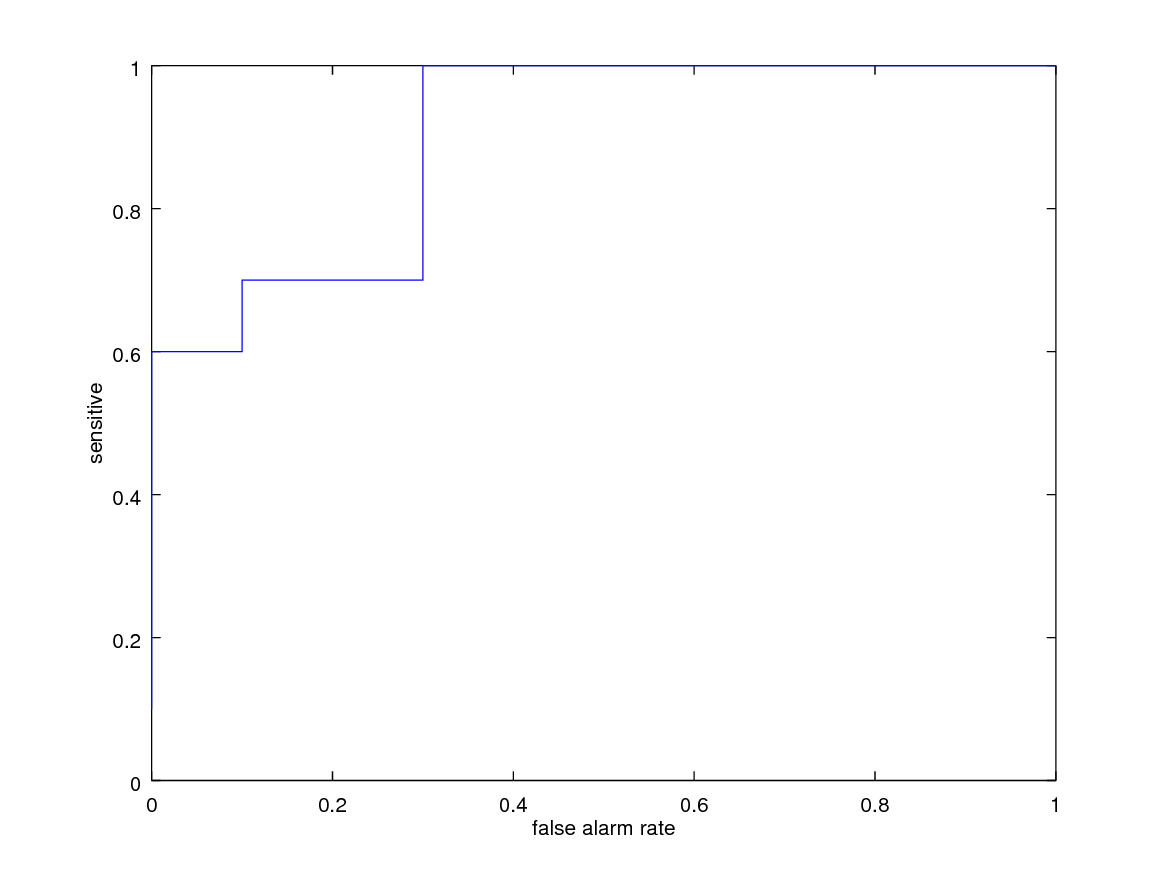
\includegraphics[scale=0.75]{result.png}
	\end{flushleft}
	\color{red}
	\item[] AUC(area under curve)=0.900
	\end{enumerate}
	
	
\end{document} 